\documentclass[a4paper, 12pt]{article}
\usepackage[total={17cm,25cm}, top=2.5cm, left=2.5cm, right=2.5cm,  includefoot]{geometry}
\usepackage[utf8]{inputenc}
\usepackage{array}
\usepackage{multirow}
\usepackage{hhline}
\usepackage{gensymb}
\usepackage{graphicx}
\graphicspath{ {} }
\usepackage[czech]{babel}
\usepackage{enumitem}
\usepackage{pdfpages}
\usepackage{amsmath}
\usepackage{verbatim}
\usepackage{listings}
\usepackage{hyperref}
\usepackage{amssymb}


\pagestyle{empty} % vypne číslování stránek




\usepackage[OT2,OT1]{fontenc}
\newcommand\cyr
{
\renewcommand\rmdefault{wncyr}
\renewcommand\sfdefault{wncyss}
\renewcommand\encodingdefault{OT2}
\normalfont
\selectfont
}
\DeclareTextFontCommand{\textcyr}{\cyr}
\def\cprime{\char"7E }
\def\cdprime{\char"7F }
\def\eoborotnoye{\char’013}
\def\Eoborotnoye{\char’003}


\begin{document}



\begin{titlepage}
\begin{center}
\noindent
\Large \textbf{České vysoké učení technické v Praze }\\ Fakulta stavební
\vspace{5cm}

\huge

%vložení loga cvut
%\begin{figure}[h!]
%	\centering
%	\includegraphics[width=7cm]{logo.png}
%\end{figure}

\vspace{0.5cm}

155ADKG: Konvexní obálky \\

\vspace{10cm}




\Large
Michael Kala\\
Anna Zemánková \\

\end{center}

\end{titlepage}




\pagestyle{plain}     % zapne obyčejné číslování
\setcounter{page}{1}  % nastaví čítač stránek znovu od jedné

%\tableofcontents
%\newpage

\section{Zadání}
Navrhněte aplikaci s grafickým rozhraním, která určí a vizualizuje konvexní obálku množiny bodů.
Pro výpočet konvexní obálky použijte algoritmy Jarvis Scan, Quick Hull a Sweep Line.\\

Pro testování algoritmů užijte rozložení bodů: \\
1) náhodné\\
2) mřížka\\
3) kružnice\\ 

\vspace{5cm}

\section{Údaje o bonusových úlohách}
V rámci této úlohy byly zpracovány všechny bonusy kromě generování star-shaped množiny bodů.\\



\clearpage

\section{Popis a rozbor problému}

Mějme množinu $S$ bodů $P_i [x_i, y_i]$, naším úkolem je nalézt konvexní obálku $\kappa$ této množiny.\\
  
Konvexní obálka $\kappa$ je hranice nejmenší kovexní množiny obsahující všechny body. \\
Pokud mezi počátečním a koncovým bodem přímého segmentu konvexní obálky leží více bodů , jde o konvexní obálku, pokud jsou odstraněny, jde o striktně konvexní obálku. \\
Např.:
\begin{itemize}
\item Konvexní obálka: A,C,D,B,E,F,G
\item Striktně konvexní obálka: A,B,E,F,G
\end{itemize}
%OBRÁZEK
\begin{figure}[h]
	\centering
	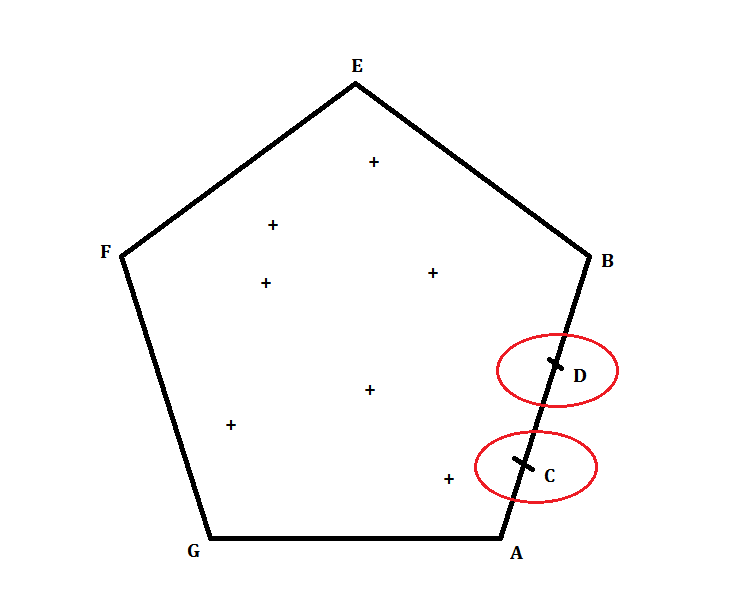
\includegraphics[width=10cm]{KO.png}
	\caption{Konvexní obálka}
\end{figure}


\clearpage
\section{Popis algoritmů}

Pro tuto úlohu byly pro výpočet konvexní obálky vybrány algortimy Jarvis Scan, Graham Scan, Quick Hull a Sweep Line.\\

\subsection{Jarvis Scan}
Tento algoritmus nejprve vybere pivota $q: y_{min}$ a následně jej přidá do konvexní obálky, poté je vybrán bod $p_{j-1}$ tak, aby spojnice pivota a $p_{j-1}$ byla rovnoběžná s osou X $p_{j-1}: x_{min}, y_{min}$ Kvůli numerické stabilitě je vybrána minimální souřadnce X z celé množiny bodů. \\
Poté je v cyklu vybírán a následně přidáván do konvexní obálky bod $p_j+1$ tak, aby byl $sphericalangle (p_{j-1}, p_j, p_{j+1})$ největší (v prvním kroku $p_j = q$). Cyklus skončí,jakmile dojde opět k pivotovi.
\vspace{1.5cm}
\subsubsection{Implementace metody}
\begin{enumerate}
\item Nalezení pivota q:  $ q = y_{min} $ 
\item Přidej $ q \longrightarrow \kappa $ 
\item Inicializuj: $p_{j-1} \in X, p_j = q, p_{j+1} = p_{j-1}$
\item Opakuj, dokud $p_{j+1} != q: $
\item 	\hspace {1cm} Nalezni $p_j+1 = argmax_{pi \in P} \measuredangle (p_{j-1}, p_j, p_i)$
\item 	\hspace {1cm} Přidej $p_j+1 \longrightarrow \kappa $
\item 	\hspace {1cm} $p_{j-1} = p_j; p_j = p_{j+1}$
\clearpage
\end{enumerate}

\subsubsection{Problematické situace}
Jestliže se ve vstupních datech vyskytují kolineární body $p_k, p_l$ (např. grid), pak může nastat:  $\sphericalangle (p_{j-1}, p_j, p_k) = \sphericalangle (p_{j-1}, p_j, p_l)$. Je tedy nutné přidat podmínku, aby byl do konvexní obálky zahrnut bod, jehož vzdálenost od bodu $p_j$ je větší.

\begin{enumerate}
\item if ($\omega_k = \omega_l$):
\item \hspace{1cm} if ($||p_j, p_k||$ $>||p_j ,p_l||$):
\item \hspace{2cm} $\kappa \longleftarrow p_k$
\item \hspace{1cm} else:
\item \hspace{2cm} $\kappa \longleftarrow p_l$
\end{enumerate}

% (OBRÁZEK)
\begin{figure}[h]
	\centering
	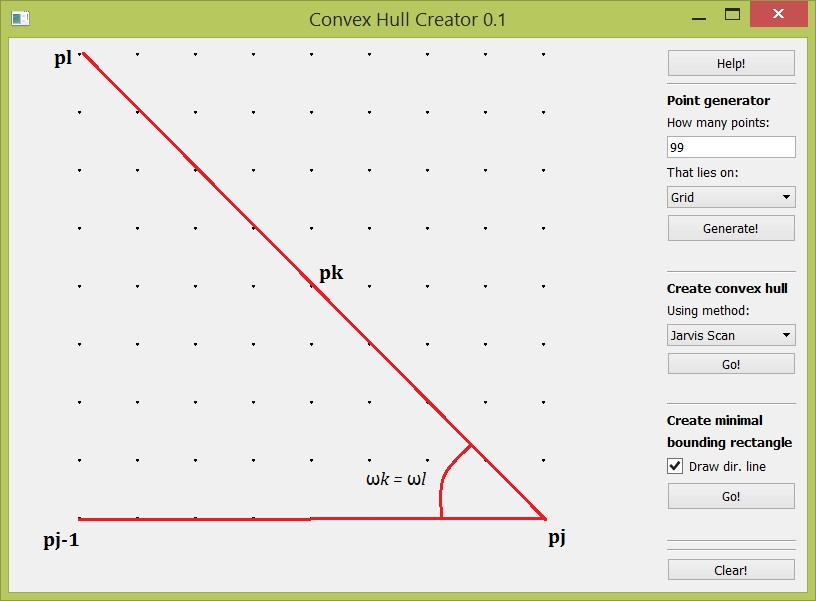
\includegraphics[width=10cm]{JS.jpg}
	\caption{Kolineární body}
\end{figure}
\clearpage
% =========================================================================================
\subsection{Graham Scan}
Nejprve je vybrán pivot $q$ tak, aby z něj bylo vidět na všechny zbylé body. Bodem q je vedena rovnoběžka s osou X a jsou určeny úhly $\omega$ od osy X po všechny ostatní body množiny. Následně jsou setříděny podle velikosti $\omega$ a pospojovány  v tomto pořadí, Vznikne tak star-shaped polygon.\\
Do zásobníku je přidán bod $q$ a první následující bod, tedy druhý. Poté je testován třetí bod - pokud je splněna podmínka levotočivosti, je přidán do zásbníku. Následně je testován čtvrtý bod. Je-li splněna podmínka levotočiosti, je přidán do zásobníku. Není-li podmínka splněna, je poslední bod v zásobníku smazán a je testován čtvrtý bod z druhého bodu atd. Po skončení cyklu je v zásobníku konvexní obálka množiy bodů.\\

\subsubsection{Implementace metody}
\begin{enumerate}
	\item Nalezení pivota q:  $ q = y_{min} $ 
	\item Setřídění $ p_i \in S$  dle $\omega_i = \measuredangle (p_i, q, x)$, index j odpovídá jejich setříděnému pořadí
	\item Pokud $\omega_k$ = $\omega_l$ , vymaž bod $p_k,p_l$ bližší ke $q$
	\item Inicialiuj $j = 2, S = \emptyset$
	\item $S \longleftarrow q, S \longleftarrow p_1$ (indexy posledních dvou prvků $p_t, p_{t-1}$) 
	\item Opakuj pro $j < n:$
	\item \hspace {1cm} if $p_j$ vlevo od $p_{t-1}, p_t:$
	\item \hspace {1.5cm} $S \longleftarrow p_j $
	\item  \hspace {1.5cm} $j = j + 1$
	\item \hspace {1cm} else pop $S$	
\end{enumerate}


\clearpage

\subsection{Quick Hull}
Algoritmus Quick Hull je rekurzivní a skládá se tedy s lokální a globální procedury.\\
V lokální proceduře je hledán nejvzdálenější bod od dělicí přímky, který zároveň leží v její pravé polorovině. Spojnici tohoto bodu a koncového bodu dělicí přímky nazývejme první segment a spojnici vyhledaného body a počátečního bodu dělicí přímky druhý segment. Aby byly body do konvexní obálky přidány ve správném pořadí, je nejprve provedena rekurze pro první segment, následně přidán vyhledaný bod a poté provedena rekurze pro druhý segment.

V globální proceduře je z množiny $S$ nalezen počáteční $p_s$ ($x_min$) a koncový $p_e$ ($x_max$) bod, které tvoří dělící přímku. Nejprve je do konvexní obálky přidán koncový bod dělicí přímky, následně je provedena lokální procedura pro horní polorovinu dělicí přímky, přidán počáteční bod dělicí přímky a  provedena lokální procedura pro dolní polorovinu. Takto dostaneme body konvexní obálky ve správném pořadí.

\subsubsection{Implementace metody - lokální procedura}
\begin{enumerate}
	\item Najdi bod $p = arg max_{pi \in S} ||p_i - (p_s, p_e)||, p \in \sigma_r (p_s, p_e)$
	\item If $ p\neq\emptyset:$,
	\item \hspace {1cm} QuickHull ($s,i,S,\kappa$) // Upper Hull
	\item \hspace {1cm} $\kappa \longleftarrow p$
	\item \hspace {1cm} QuickHull ($i,e,S,\kappa$) // Lower Hull
\end{enumerate}

\subsubsection{Implementace metody - globální procedura}

\begin{enumerate}
	\item  $\kappa = \emptyset, S_U = \emptyset S_L \emptyset$
	\item $q_1 = x_{min}, q_3 = x_{max}$
	\item $S_U \longleftarrow q_1$, $S_U \longleftarrow q_3$
	\item $S_L \longleftarrow q_1$, $S_L \longleftarrow q_3$
	\item for $p_i \in S$
	\item \hspace {1cm} if ($p_i \in \sigma_l (q_1, q_3)$) $S_U \longleftarrow p_i$
	\item \hspace {1cm} else $S_L \longleftarrow p_i$
	\item $\kappa \longleftarrow q_3$
	\item QuickHull ($1,0,S_U,\kappa$) // Upper Hull
	\item $\kappa \longleftarrow q_1$
	\item QuickHull ($0,1,S_L,\kappa$) // Lower Hull
\end{enumerate}
\clearpage

\subsubsection{Prolematické situace}
Problematická situace při využití algotimu Quick Hull nastává v okamžiku, kdy je vstupní množina uspořádána do kružnice. Spojnice počátečního $p_s$ a koncového bodu $p_e$ je pak vždy sečna kružnice -> existuje další bod v pravé polorovině dokud do konvexní obálky nejsou zařazeny všechny body a rekurze bude volána pro každý bod vstupní množiny. V obrázku níže jsou naznačeny první tři kroky, odlišené barvami.

% (OBRÁZEK)
\begin{figure}[h]
	\centering
	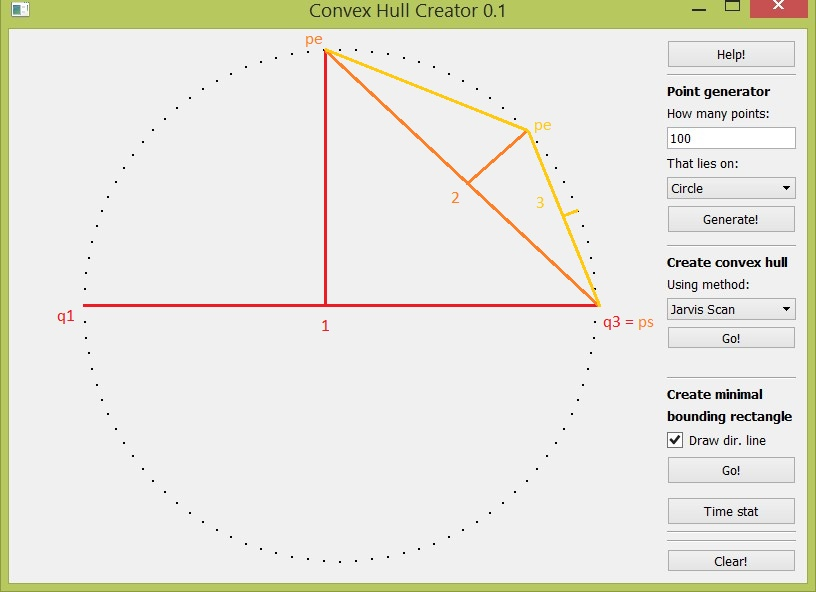
\includegraphics[width=10cm]{circle.jpg}
	\caption{Quick Hull - kružnice}
\end{figure}
\clearpage

\clearpage
\subsection{Sweep Line}
Metoda sweep line pracuje s "přepisováním" předchůdců a  následníků a jelikož by se tu až nezdravě opakovala slova přechůdce a následník, samotná implementace metody bude srozumitelnější (jako ostatně vždy).

\subsubsection{Implementace metody}
\begin{enumerate}
	\item  Sort $P_s = sort (P)$ by x
	\item if $p_3 \in \sigma_L (p_1, p_2)$
	\item \hspace {1cm} n[1] = 2; n[2] = 3; n[3] = 1
	\item \hspace {1cm} p[1] = 3; p[2] = 1; p[3] = 2
	\item else
	\item \hspace {1cm} n[1] = 3; n[3] = 2; n[2] = 1
	\item \hspace {1cm} p[1] = 2; p[3] = 1; p[2] = 3
	\item for $p_i \in P_s, i > 3$
	\item \hspace {1cm} if ($y_i>y_i-1$) 
	\item \hspace {2cm} p[i] = i-1; n[i] = n[i-1]
	\item \hspace {1cm} else 
	\item \hspace {2cm} n[i] = i-1; p[i] = p[i-1]
	\item \hspace {1cm}n[p[i]] = i; p[n[i]] = i;
	\item \hspace {1cm}while (n[n[i]]) $\in \sigma_R (i, n[i]) $
	\item \hspace {2cm} p[n[n[i]]] = i; n[i] = n[n[i]];
	\item \hspace {1cm} while (p[p[i]]) $\in \sigma_L (i, p[i]) $
	\item \hspace {2cm} n[p[p[i]]] = i; p[i] = p[p[i]];
\end{enumerate}
\clearpage

\subsection{Minimální ohraničující obdélník}
Pro výpočet minimálního ohraničující obdélníku byl vybrán následující algoritmus. Na jeho vstupu je konvexní obálka ch.

\subsubsection{Implementace metody}
\begin{enumerate}

	\item for $p_{i\%n}, p_{(i+1)\%n} \in ch$ //n = ch.size
	\item \hspace{1cm} rotuj ch o $\sphericalangle (|p_{i\%n}, p_{(i+1)\%n}| , ||$ s osou x)
	\item \hspace{1cm} najdi nejmenší resp. největší x a y souřadnice, spočti obsah jimi vytvořeného obdélníka, pokud je menší než jakýkoliv doposud vypočtený, ulož ho, ulož úhel, o který bylo rotováno, ulož souřadnice 
	\item \hspace{1cm} rotuj zpět o úhel z kroku 2
	\item rotuj zpět souřadnice obdélníka o uložený úhel	
	
\end{enumerate}

\vspace{1,5cm}


\subsection{Striktně konvexní obálka}
Jak již bylo řečeno výše, striktně konvexní obálka na přímém segmentu neobsahuje žádné jiné body kromě počátečního a koncového bodu segmentu. Pro odstranění mezilehlých bodů byla vypočtena rovnice přímky prvních dvou bodů. Poté byl do rovnice dosazen bod třetí, pokud ležel na přímce, byl odstraněn z konvexnní obálky. Neležel-li na přímce, byla vypočtena rovnice přímky druhého a třetího bodu a poté do ní byl dosazen bod čtvrtý atd. Cyklus končí jakmile je ověřen poslední bod konvexní obálky.

\subsubsection{Implementace metody}
\begin{enumerate}
	
	\item 	
	
\end{enumerate}

\clearpage

\section{Vstupní data}

Vstupními daty je množina bodů, kterou lze zadat dvěma způsoby:\\
1) klikáním na kanvas\\
2) použitím generátoru bodů, který je součástí aplikace, přičemž se body generují dle zadaných kritérií.\\


 Do generátoru bodů je třeba zadat počet bodů a následně vybrat v rozbalovacím menu 
 požadované rozmístění - Random/Grid/Circle/Elipse/Square 

%OBRÁZEK
\begin{figure}[h]
	\centering
	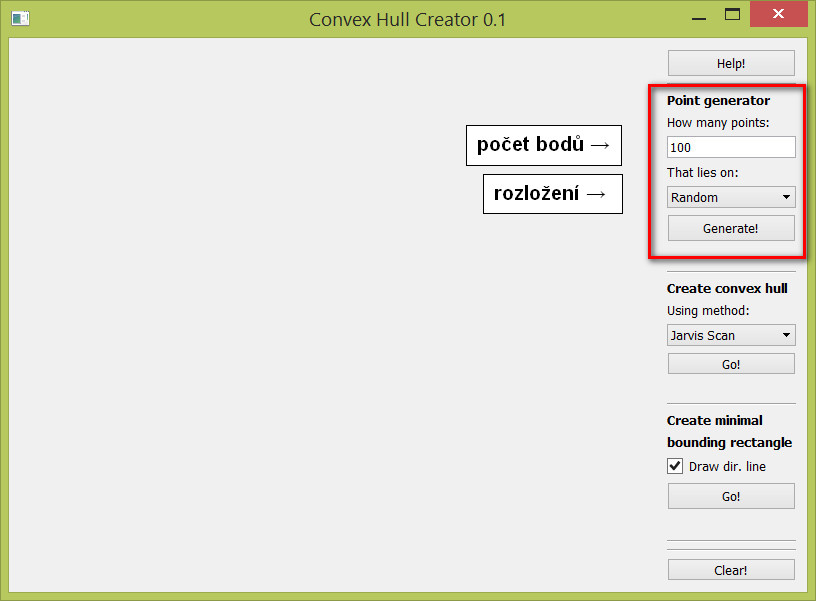
\includegraphics[width=10cm]{vstup_nastaveni.jpg}
	\caption{Generátor bodů}
\end{figure}
 
V případě, že je zadán nekorektní počet bodů pro dané rozmístění - např. pro čtverec nebo grid, je obrazen vytvořen z nejbližšího menšího možného počtu prvků.

%OBRÁZEK
\begin{figure}[h]
	\centering
	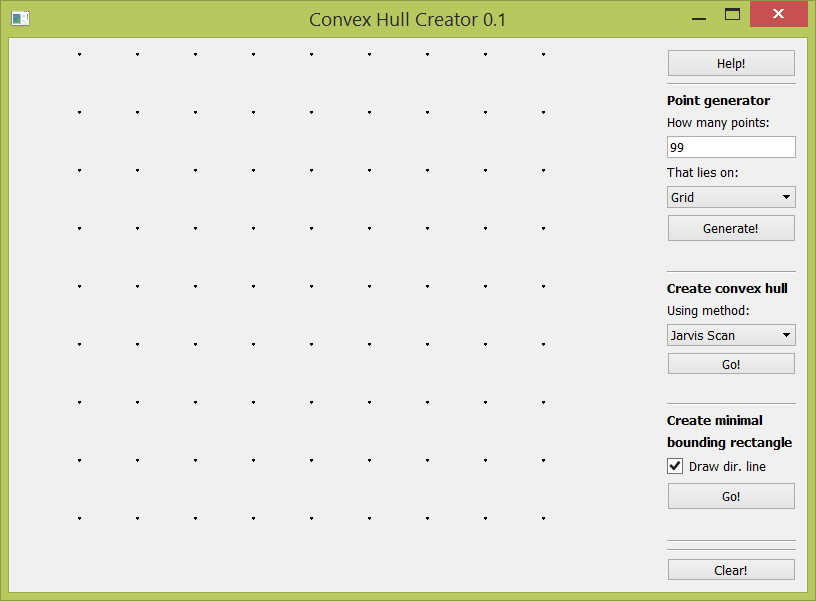
\includegraphics[width=10cm]{vstup.jpg}
	\caption{Ukázka nekorektního počtu bodů pro zadaný tvar}
\end{figure}
 
Pokud jsou body vygenerovány pomocí generátoru, je možné přidat další klikáním na kanvas.
Při špuštění generátoru jsou všechny dosud existující body vymazány.

\clearpage
\section{Výstupní data}
Výsledná data (konvexní obálka/minimální ohraničující obdélkník/hlavní směr útvaru) jsou vizualizována v kanvasu aplikace.   \\
% (OBRÁZEK)
\begin{figure}[h]
	\centering
	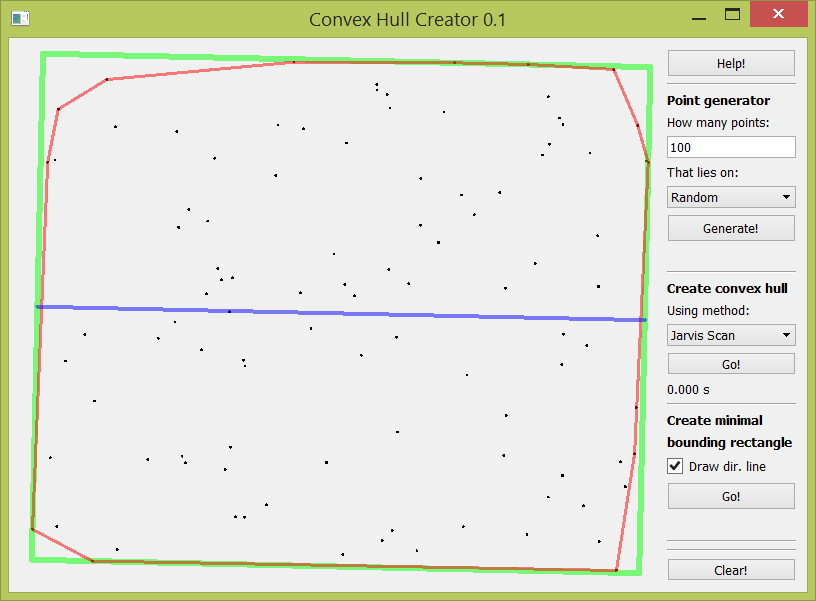
\includegraphics[width=10cm]{min_bound.jpg}
	\caption{Výstupní data}
\end{figure}

%--------------------------------------------------------------------------------------------------------------------------------------

\clearpage
\section{Ukázka vytvořené aplikace}
\begin{figure}[h!]
	\centering
	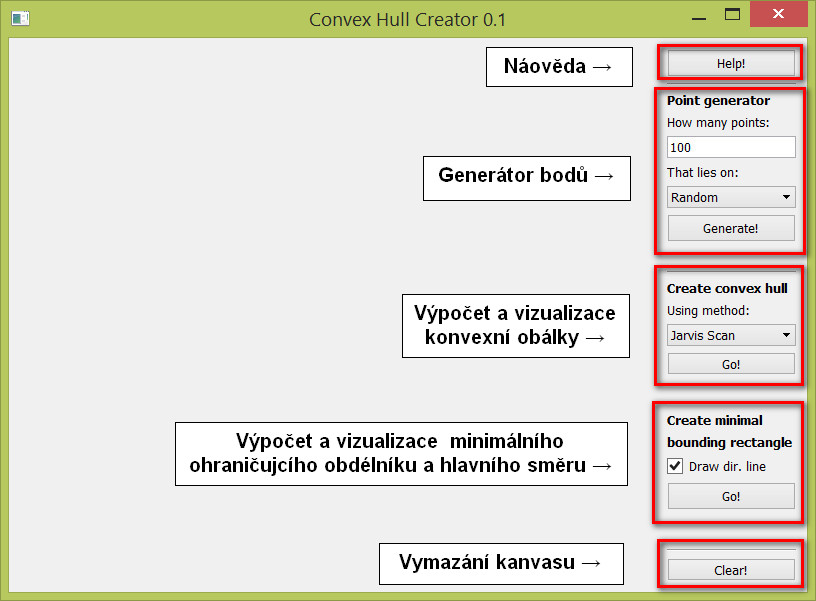
\includegraphics[width=10cm]{popis.jpg}
	\caption{Okno aplikace}
\end{figure}

V Pravé horní části je možnost kliknutí na nápovědu "Help", poté se otevře okno s nápovědou, 
kde je popsán způsob zadávání vstupních dat a funkcionality aplikace.\\

% (OBRÁZEK)
\begin{figure}[h!]
	\centering
	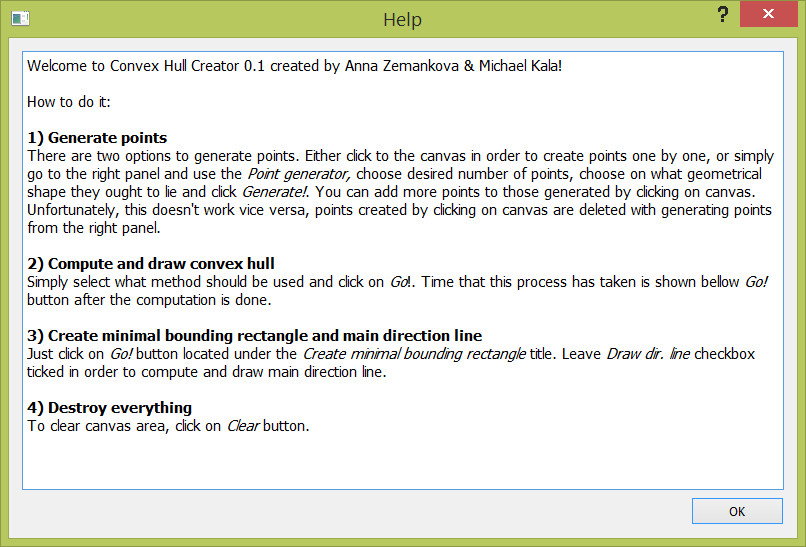
\includegraphics[width=10cm]{help.jpg}
	\caption{Nápověda}
\end{figure}

\clearpage


Nejprve je třeba zadat vstupní data - množinu bodů.\\
% (OBRÁZEK)
\begin{figure}[h!]
	\centering
	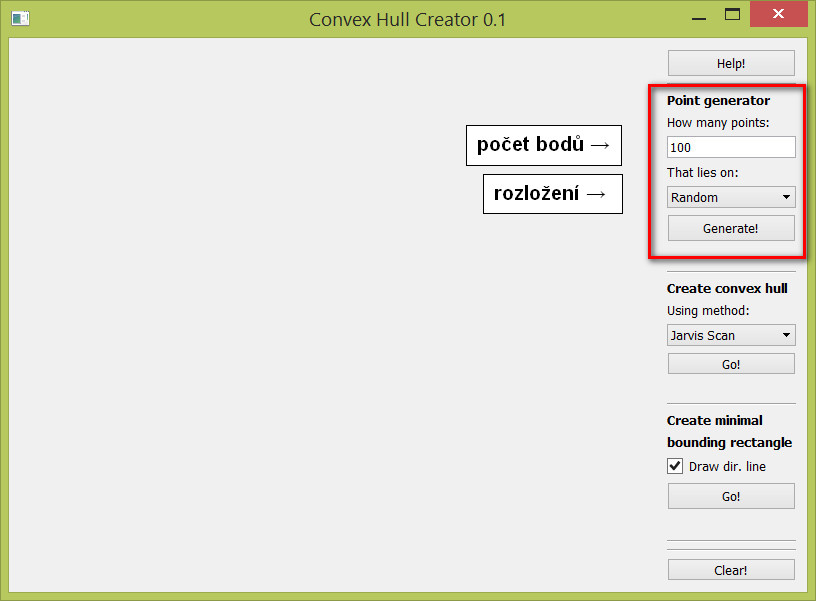
\includegraphics[width=10cm]{vstup_nastaveni.jpg}
	\caption{Vstupní data}
\end{figure}

Následně je možné vybrat metodu výpočtu konvexní obálky a kliknutím na tlačítko GO v 
sekci Create convex hull zahájen výpočet a vizualizace konvexní obálky zadané množiny bodů.
Pod tlačítkem Go je vypsán čas, jak dlouho trval výpočet.\\
% (OBRÁZEK)
\begin{figure}[h!]
	\centering
	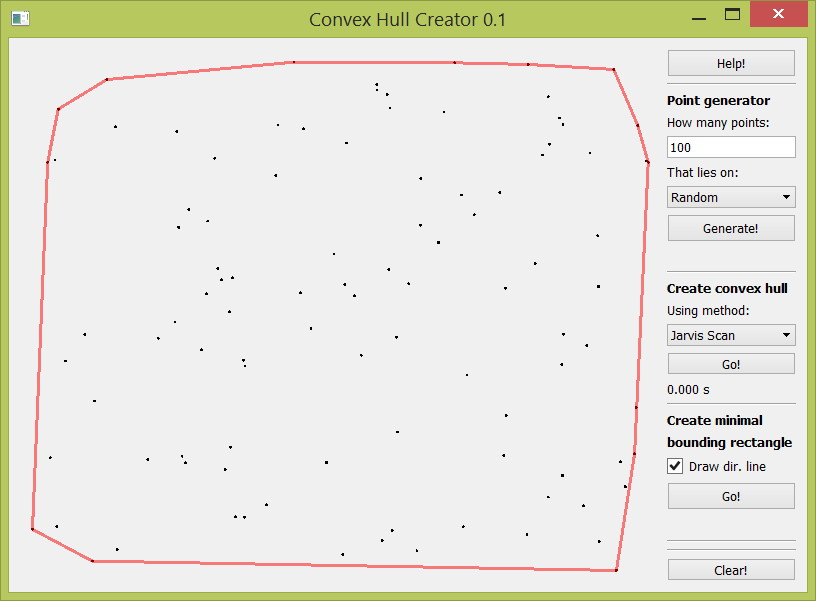
\includegraphics[width=10cm]{vystup.jpg}
	\caption{Výpočet konvexní obálky}
\end{figure}


Pokud chceme spočítat minimální ohraničující obdélník, lze tak učinit kliknutím
 na tlačítko Go! v sekci  Create inimal bounding rectangle. Pokud je v této sekci
 zaškrtnuta možnost draw dir. line, vykreslí se také hlavní směr útvaru.\\
% (OBRÁZEK)
\begin{figure}[h!]
	\centering
	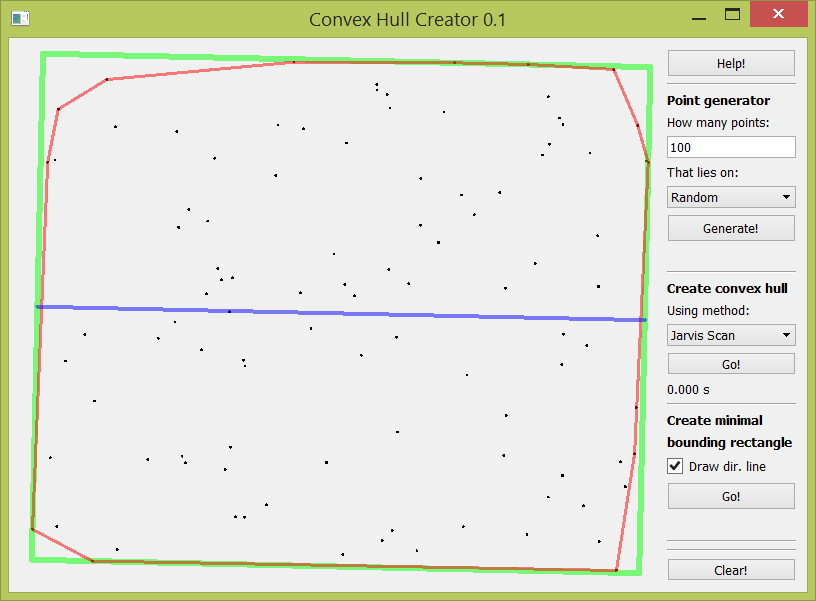
\includegraphics[width=10cm]{min_bound.jpg}
	\caption{Výpočet hlavního směru a nejmenšího ohraničujícícho obdélníku}
\end{figure}

Vše je uvedeno do původního stavu (smazány body i vypočtené vyýsledky) kliknutím na tlačítko Clear.\\

\clearpage

%=======================================================================================
\section{Testování výpočetních dob algoritmů}
V rámci této úlohy byly testovány výpočetní doby algoritmů pro vsutpní množim o počtu bodů 1 000 - 1 000 000 bodů. Pro každý interval a každý tvar vstupní množiny byl výpočet proveden 10x, následně byl určen průměr a rozptyl. \\
Na základě těchto testování bylo zjištěno, že algoritmy Sweep Line a Quick Hull jsou univerzální výpočetní algoritmy konvexní obálky pro různé uspořádání množiny bodů a to i pro velké množiny bodů. Graham Scan je oproti nim vždy (kromě kružnice) o řád až dva pomalejší. Jarvis Scan s ostatními algoritmy snad ani nelze srovnávat – je vždy o několik řádů pomalejší. 
Níže jsou uvedeny výsledné průměrné hodnoty a jejich grafy. Podrobnější záznam testování viz přílohu č. 1 "Testování".

\vspace{1.5cm}
\subsection {Rozložení bodů - random}
% (OBRÁZEK)
\begin{figure}[h!]
	\centering
	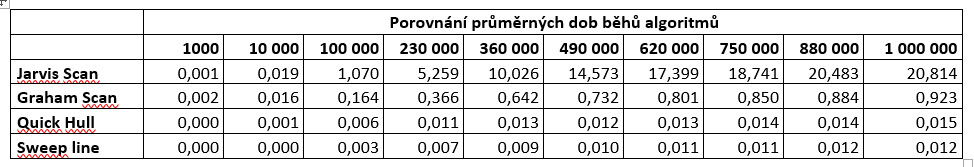
\includegraphics[width=15cm]{random.jpg}
	\caption{Porovnání průměrné doby výpočtu - random}
\end{figure}


\begin{figure}[h!]
	\centering
	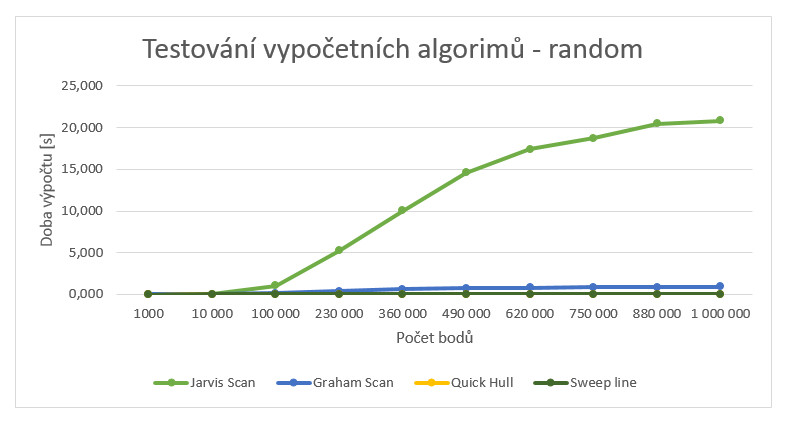
\includegraphics[width=12cm]{g1_random.jpg}
	\caption{Graf porovnání průměrné doby výpočtu - random}
\end{figure}
\clearpage

Pro vizuální porovnání algoritmů Quick hull, Sweep line a Graham scan byl vytvořen graf zvlášť.
\begin{figure}[h!]
	\centering
	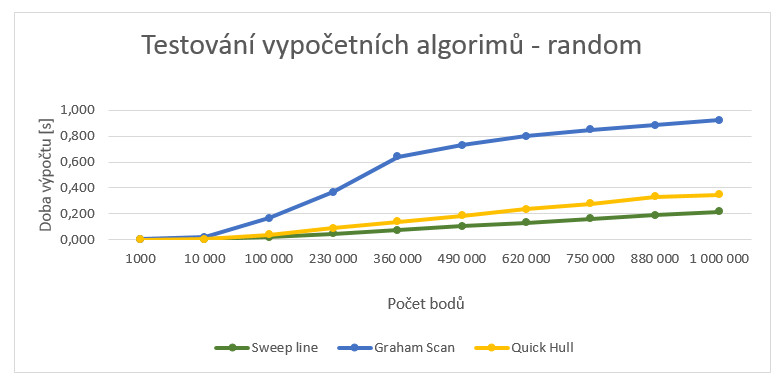
\includegraphics[width=12cm]{g2_random.jpg}
	\caption{Graf porovnání průměrné doby výpočtu - random}
\end{figure}

\subsection {Rozložení bodů - grid}
% (OBRÁZEK)
\begin{figure}[h!]
	\centering
	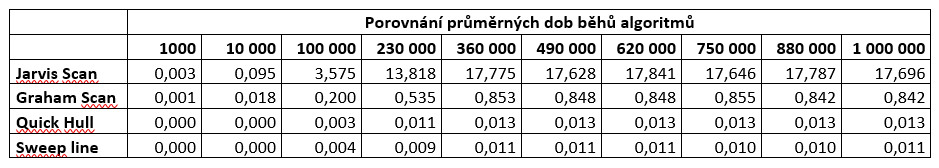
\includegraphics[width=15cm]{grid.jpg}
	\caption{Porovnání průměrné doby výpočtu - grid}
\end{figure}


\begin{figure}[h!]
	\centering
	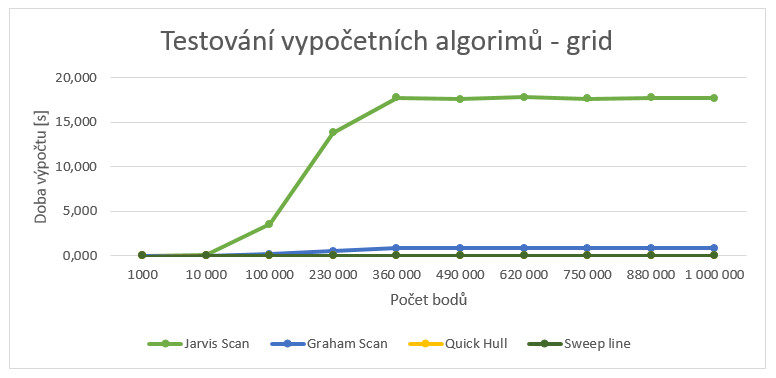
\includegraphics[width=12cm]{g1_grid.jpg}
	\caption{Graf porovnání průměrné doby výpočtu - grid}
\end{figure}
\clearpage

Pro vizuální porovnání algoritmů Quick Hull a Sweep Line byl vytvořen graf zvlášť.
\begin{figure}[h!]
	\centering
	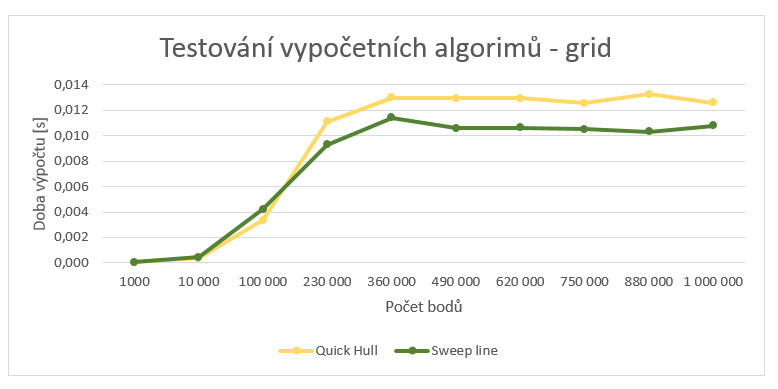
\includegraphics[width=12cm]{g2_grid.jpg}
	\caption{Graf porovnání průměrné doby výpočtu - grid}
\end{figure}
\subsection {Rozložení bodů - circle}

% (OBRÁZEK)
\begin{figure}[h!]
	\centering
	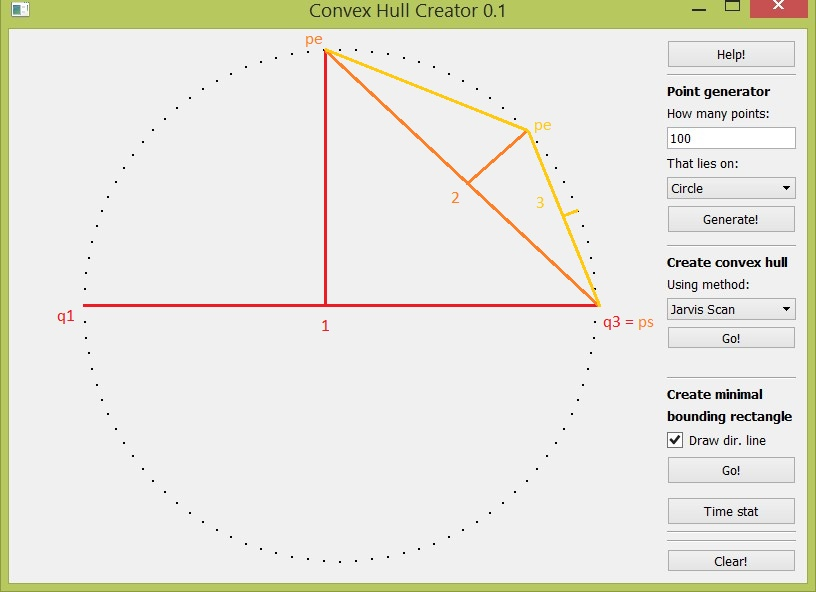
\includegraphics[width=15cm]{circle.jpg}
	\caption{Porovnání průměrné doby výpočtu - circle}
\end{figure}


\begin{figure}[h!]
	\centering
	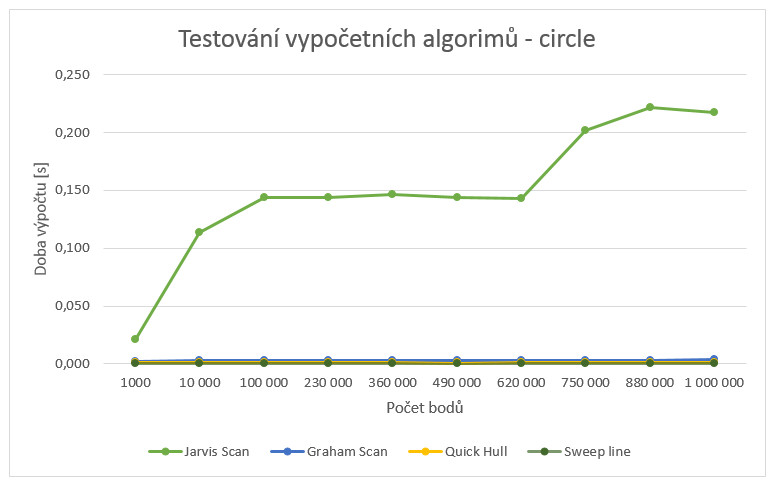
\includegraphics[width=12cm]{g1_circle.jpg}
	\caption{Graf porovnání průměrné doby výpočtu - circle}
\end{figure}
\clearpage

Pro vizuální porovnání algoritmů Quick Hull, Sweep Line a Graham scan byl vytvořen graf zvlášť.
\begin{figure}[h!]
	\centering
	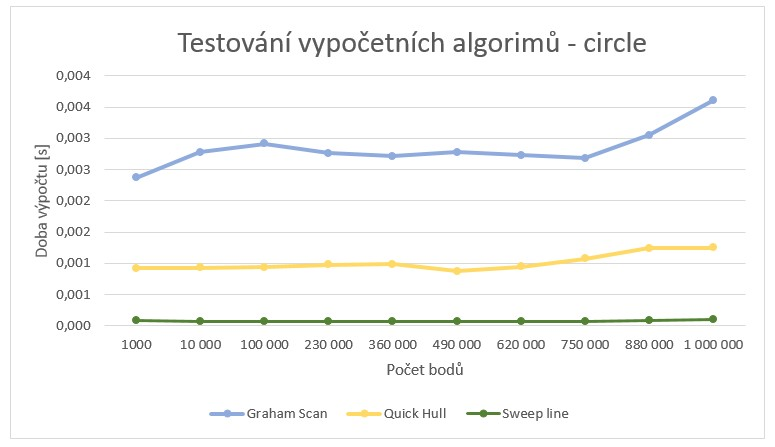
\includegraphics[width=12cm]{g2_circle.jpg}
	\caption{Graf porovnání průměrné doby výpočtu - circle}
\end{figure}
\clearpage
\section{Dokumentace}

\subsection{Algorithms}
V třídě Algorithms jsou staticky implementovány algoritmy počítající kovexní obálku a minimální ohraničující obdélník (včetně vodící linie).

\begin{itemize}

	\item Výčtový typ \textbf{TPosition}
		\begin{itemize}
			\item Typ využitý jako návratová hodnota členské metody \textbf{getPointLinePosition}.
			\item \textbf{LEFT = 0}
			\item \textbf{RIGHT = 1}
			\item \textbf{ON = 2}
		\end{itemize}

	\item Metoda \textbf{getPointLinePosition}
		\begin{itemize}
			\item Tato metoda slouží k určení polohy bodu vůči přímce. Návratovou hodnotou je výčtový typ \textbf{TPosition}.
			\item Vstup
				\begin{itemize}
					\item \textbf{QPointF \&q} - určovaný bod
					\item \textbf{QPointF \&a, \&b} - body přímky
				\end{itemize}
			\item Výstup
				\begin{itemize}
					\item \textbf{LEFT} - bod vlevo od přímky
					\item \textbf{RIGHT} - bod vpravo od přímky
					\item \textbf{ON} - bod na přímce
				\end{itemize}

		\end{itemize}

	\item Metoda \textbf{getTwoVectorsAngle}
		\begin{itemize}
			\item Tato metoda slouží k určení úhlu mezi 2 přímkami. Její návratovou hodnotu je \textbf{double}.
			\item Vstup
				\begin{itemize}
					\item \textbf{QPointF \&p1, \&p2} - body první přímky
					\item \textbf{QPointF \&p3, \&p4} - body druhé přímky
				\end{itemize}
		
			\item Výstup
				\begin{itemize}
					\item Úhel mezi 2 přímkami
				\end{itemize}			
		\end{itemize}

	\item Metoda \textbf{getPointLineDistance}
		\begin{itemize}
			\item Tato metoda slouží k výpočtu vzdálenosti bodu od přímky. Její návratovou hodnotou je \textbf {double} %\begin{double.}
			\item Vstup
				\begin{itemize}
					\item \textbf{QPointF \&q} - určovaný bod
					\item \textbf{QPointF \&a, \&b} - body přímky
				\end{itemize}
			\item Výstup
				\begin{itemize}
					\item Vzdálenost bodu od přímky
				\end{itemize}
		\end{itemize}

	\item Přetížená metoda \textbf{rotateByAngle}
		\begin{itemize}
			\item Tato metoda slouží k rotaci dané množiny o úhel. Jejím návratovým typem je \textbf{void}.
			\item Vstup
				\begin{itemize}
					\item Přetížení 1
						\begin{itemize}
							\item \textbf{std::vector$<$QPointF$>$ \&points} - vektor bodů, jež má být orotován
							\item \textbf{double angle} - úhel, o který má rotace být provedena
 						\end{itemize}
					
					\item Přetížení 2
						\begin{itemize}
							\item \textbf{QPolygonF \&points} - polygon, jež má být orotován
							\item \textbf{double angle} - úhel, o který má rotace být provedena
 						\end{itemize}

					\item Přetížení 3
						\begin{itemize}
							\item \textbf{QLineF \&points} - úsečka, jež má být orotována
							\item \textbf{double angle} - úhel, o který má rotace být provedena
 						\end{itemize}					
				\end{itemize}
			
		\end{itemize}

	\item Metoda \textbf{getDistance}
		\begin{itemize}
			\item Tato metoda slouží k výpočtu vzdálenosti dvou bodů. Jejím výstupním typem je \textbf{double}.
			\item Vstup
				\begin{itemize}
					\item \textbf{QPointF \&a, \&b} - body, mezi kterými je vzdálenost počítána
				\end{itemize}
			\item Výstup
				\begin{itemize}	
					\item Vypočtená vzdálenost
				\end{itemize}
		\end{itemize}

	\item Metoda \textbf{jarvisScanCH}
		\begin{itemize}
			\item Tato metoda slouží k výpočtu konvexní obálky pomocí algoritmu Jarvis Scan. Během výpočtu je ošetřována singularita existence kolineárních bodů v datasetu. Jejím výstupním typem je \textbf{QPolygonF}.
			\item Vstup
				\begin{itemize}
					\item \textbf{std::vector} $<$\textbf{QPointF}$>$ \textbf{points} - vektor bodů, kolem nichž má být vytvořená konvexní obálka.
				\end{itemize}
			\item Výstup
				\begin{itemize}
					\item Polygon obsahující kovexní obálku.
				\end{itemize} 
		\end{itemize}

	\item Metoda \textbf{grahamScanCH}
		\begin{itemize}
			\item Tato metoda slouží k výpočtu konvexní obálky pomocí algoritmu Graham Scan. Jejím výstupním typem je \textbf{QPolygonF}.
			\item Vstup
				\begin{itemize}
					\item \textbf{std::vector} $<$\textbf{QPointF}$>$ \textbf{points} - vektor bodů, kolem nichž má být vytvořená konvexní obálka.
				\end{itemize}
			\item Výstup
				\begin{itemize}
					\item Polygon obsahující kovexní obálku.
				\end{itemize} 
		\end{itemize}

	\item Metoda \textbf{quickHullCH}
		\begin{itemize}
			\item Tato metoda slouží k výpočtu konvexní obálky pomocí algoritmu Quick Hull. Jejím výstupním typem je \textbf{QPolygonF}.
			\item Vstup
				\begin{itemize}
					\item \textbf{std::vector} $<$\textbf{QPointF}$>$ \textbf{points} - vektor bodů, kolem nichž má být vytvořená konvexní obálka.
				\end{itemize}
			\item Výstup
				\begin{itemize}
					\item Polygon obsahující kovexní obálku.
				\end{itemize} 
		\end{itemize}

	\item Metoda \textbf{quickHullLocal}
		\begin{itemize}
			\item Pomocná metoda k výpočtu konvexní obálky metodou Quick Hull. Jejím výstupním typem je \textbf{void}.
			\item Vstup
				\begin{itemize}
					\item \textbf{int s, e} - index počátečního a koncového bodu dělící přímky
					\item \textbf{std::vector} $<$\textbf{QPointF}$>$ \&\textbf{points} - vektor bodů, kolem nichž má být vytvořená konvexní obálka.
					\item \textbf{QPolygonF \&poly\_ch} - polygon obsahující body konvexní obálky
				\end{itemize}
			\item Výstup
				\begin{itemize}
					\item Polygon obsahující kovexní obálku.
				\end{itemize} 
		\end{itemize}

	\item Metoda \textbf{sweepLineCH}
		\begin{itemize}
			\item Tato metoda slouží k výpočtu konvexní obálky pomocí algoritmu Sweep Line. Jejím výstupním typem je \textbf{QPolygonF}.
			\item Vstup
				\begin{itemize}
					\item \textbf{std::vector} $<$\textbf{QPointF}$>$ \textbf{points} - vektor bodů, kolem nichž má být vytvořená konvexní obálka.
				\end{itemize}
			\item Výstup
				\begin{itemize}
					\item Polygon obsahující kovexní obálku.
				\end{itemize} 
		\end{itemize}

	\item Metoda \textbf{generatePoints}
		\begin{itemize}
			\item Metoda pro generování zadaného počtu a tvaru bodů. Jejím výstupním typem je \textbf{std::vector} $<$\textbf{QPointF}$>$ \textbf{points}.
			\item Vstup
				\begin{itemize}
					\item \textbf{QSizeF \&canvas\_size} - rozměry kreslícího plátna, ze kterých se determinuje rozsah generovaných bodů
					\item \textbf{int point\_count} - počet bodů, který se má generovat
					\item \textbf{std::string shape} - tvar vytvářené množiny bodů (random, grid, na kružnici, na elipse, na čtverci)
				\end{itemize}
			\item Výstup
				\begin{itemize}
					\item Vektor nagenerovaných bodů.
				\end{itemize}
		\end{itemize}

	\item Metoda \textbf{minimalRectangle}
		\begin{itemize}
			\item Metoda pro výpočet minimálního ohraničujícího obdélníku a hlavní linie. Jejím výstupním typem je \textbf{void}.
			\item Vstup
				\begin{itemize}
					\item \textbf{QPolygonF \&poly\_ch} - polygon obsahující konvexní obálku
					\item \textbf{QPolygonF \&minimal\_rectangle} - polygon, do kterého jsou počítány body minimálního ohraničujícího obdélníku
					\item \textbf{QLineF \&direction} - hlavní linie minimálního ohraničujícího obdelníku (resp. do této proměnné je počítaná)
					\item \textbf{bool compute\_dir\_line} - ukazatel určující zda-li má být počítána hlavní linie minimálního ohraničujícího obdélníku
				\end{itemize}

		\end{itemize}
\end{itemize}
\clearpage

\subsection{Draw}
Třída draw slouží k vykreslení vygenerovaných (nebo naklikaných) bodů, vypočteného minimálního ohraničujícího obdélníku a hlavní linie minimálního ohraničujícího obdélníku. V této třídě jsou zároveň nagenerované body zbavené duplicit a vypočtené konvexní obálky se zde omezují na striktní konvexní obálky (vše v metodě \textbf{setCH}. Třída dědí od třídy \textbf{QWidget}. 

\begin{itemize}
	\item Členské proměnné
		\begin{itemize}
			\item \textbf{std::vector} $<$\textbf{QPointF}$>$ \textbf{points} - vektor obsahující nagenerované nebo naklikané body
			\item \textbf{QPOlygonF ch} - polygon obsahující body konvexní obálky
			\item \textbf{QPolygonF rect} - polygon obsahující body minimálního ohraničujícího obdélníku
			\item \textbf{QLineF direction} - hlavní linie minimálního ohraničujícího obdélníka
		\end{itemize}

	\item Metoda \textbf{paintEvent}
		\begin{itemize}
			\item Tato metoda slouží k vykreslení nagenerovaných (nebo naklikaných) bodů, konvexní obýlky, minimálního ohraničujícího obdélníka a hlavní linie minimálního ohraničujícího obdélníka. Metoda se volá pomocí metody \textbf{repaint()}. Návratovým typem je \textbf{void}.
			\item Vstup
				\begin{itemize}
					\item \textbf{QPaintEvent *e}
				\end{itemize}
		\end{itemize}

	\item Metoda \textbf{mousePressEvent}
		\begin{itemize}
			\item Metoda sloužící k uložení bodu do členské proměnné \textbf{points} určeného kliknutím myší nad kreslícím plátnem. Jejím návratovým typem je \textbf{void}.	
			\item Vstup
				\begin{itemize}
					\item \textbf{QMouseEvent *e}
				\end{itemize}
		\end{itemize}

	\item Metoda \textbf{setCH}
		\begin{itemize}
			\item Tato metoda slouží pro kontrolu duplicity generovaných bodů, pro kontrolu alespoň 3 bodů, k zavolání příslušného algoritmu pro vypočtení konvexní obálky a k omezení konvexní obálky na striktně konvexní obálku. Metoda počítá dobu trvání výpočetních algoritmů. Jejím návratovým typem je \textbf{double}.
			\item Vstup
				\begin{itemize}
					\item \textbf{std::string \&selected\_algorithm} - uživatelsky vybraný algoritmus pro počítání konvexní obálky
				\end{itemize}
			\item Výstup
				\begin{itemize}
					\item Čas trvání výpočtu.
				\end{itemize}
		\end{itemize}	

	\item Metoda \textbf{setRect}
		\begin{itemize}
			\item Tato metoda slouží pro zavolání algoritmu pro výpočte minimálního ohraničujícího obdélníku a jeho hlavní linie. Jejím návratovým typem je \textbf{void}.
			\item Vstup
				\begin{itemize}
					\item \textbf{bool draw\_dir\_line} - uživatelsky nastavený indikátor, zda-li se má vypočítat hlavní linie minimálního ohraničujícího obdélníku
				\end{itemize}
		\end{itemize}

	\item Metoda \textbf{setPoints}
		\begin{itemize}
			\item Metoda volající algoritmus pro generování bodů daného počtu a tvaru. Jejím návratovým typem je \textbf{void}.
			\item Vstup
				\begin{itemize}
					\item \textbf{QSizeF \&canvas\_size} - rozměr kreslícího plátna pro pozdější určení rozsahu generování bodů
					\item \textbf{int count} - počet bodů, jež se má generovat
					\item \textbf{std::string \&shape} - tvar, do kterého se body mají generovat
				\end{itemize}
		\end{itemize}

	\item Metoda \textbf{clearCanvas}
		\begin{itemize}
			\item Metoda, která maže obsah kreslícího okna. Jejím návratovým typem je \textbf{void}. Do metody nevstupují žádné parametry.
		\end{itemize}
\end{itemize}

\subsection{SortByXAsc, SortByYAsc, SortByAngleAsc}
Třídy sloužící jako sortovací kritérium - podle rostoucí souřadnice x resp. souřadnice y (při stejných souřadnicích x resp. y je druhým kritériem druhá souřadnice) a podle rostoucího úhlu mezi body (při stejném úhlu je druhým kritériem vzdálenosti mezi body).
\clearpage

\subsection{Widget}
Tato třída slouží ke komunikaci s GUI. Třída dědí od třídy QWidget. Všechny její metody slouží jako sloty k signálům z GUI, nemají žádné vstupní hodnoty a jejich návratovým typem je void. 

\begin{itemize}
	\item Metoda \textbf{on\_createCHButton\_clicked} - reaguje na zmáčknutí tlačítka pro vypočtení konvexní obálky, volá metodu \textbf{setCH} z třídy \textbf{Draw}, zapisuje čas výpočtu do GUI.

	\item Metoda \textbf{on\_generateButton\_clicked} - reaguje na zmáčknutí tlačítka pro generování bodů, volá metodu \textbf{setPoints} z třídy \textbf{Draw}.

	\item Metoda \textbf{on\_clearButton\_clicked} - reaguje na zmáčknutí tlačítka pro vymazání obsahu kreslícího plátna, volá metodu \textbf{clearCanvas} z třídy \textbf{Draw}.

	\item Metoda \textbf{on\_createRectButton\_clicked} - reaguje na zmáčknutí tlačítka pro vypočtení minimálního ohraničujícího obdélníka, volá metodu \textbf{setRect} z třídy \textbf{Draw}.

	\item Metoda \textbf{on\_helpButton\_clicked} - reaguje na zmáčknutí tlačítka pro volání nápovědy, volá okno s nápovědou \textbf{help\_dialog} z třídy \textbf{HelpDialog}.

\end{itemize} 

\vspace{3cm}
\subsection{HelpDialog}
Třída sloužící pro vykreslení okna s nápovědou.

\clearpage

\section{Přílohy}

\begin{itemize}
	\item Príloha č.1: Testování výpočetních dob algoritmů - "Testovani.pdf"
\end{itemize}
 %--------------------------------------------------------------------------------------------------------------------------------------------------------------------------
\clearpage
\section{Závěr}

\subsection{Politování se a vysvětlení našeho problému}
Aplikace od začátku implementovala body, polygony, linie atd. v typu float (QPointF, QPolygonF, QLineF), v tomto duchu byly psány i všechny algoritmy. Při testování bylo zjištěno, že výpočet takto implementovaných algoritmů trvá VELMI dlouho (v řádu stovek sekund). Proto bylo navrženo (dva dny před odevzdáním), že by bylo vhodné vyzkoušet, jak budou algoritmy rychle počítat při implementaci bodů, polygonů a linií v typu int (QPoint, QPolygon, QLine). Bylo zjištěno, že tato změna (aplikovaná pomocí programu grep (to jsme se jen chtěli pochlubit, že jsme to zmákli přepsat rychle)) algoritmy rapidně urychlí (do řádu sekund až sub-sekund). Z tohoto důvodu (a také z časových důvodů, při testování pomalejší verze počítač zamrzá a člověk u toho musí pořád sedět a odklikávat "Wait", aby program nepadl) jsou uvedeny grafy z testování rychlejší verze. Kdyby všechny algoritmy po tomto přechodu fungovaly správně, ani bychom se neobtěžovali psát tak obsáhlý závěr, ale to by nebyla smůla, aby se to nerozbilo. Především myšlenka rotací tam a zpět u minimálního ohraničujícího obdélníku již nefunguje - orotované souřadnice se zaokrouhlí na celé číslo, při rotaci zpět se opět zaokrouhlí na celé číslo a problém je na světě. \\
Dále je jakýmsi neidentifikovatelným způsobem rozbitý výpočet Jarvis Scan na kružnici (kód jsme změnili na kód stejný jako z hodiny, kód generování bodů na kružnici máme obdobný jako ostatní skupinky, ale i tak nefunguje úplně správně, neumíme určit problém (a moc nás to mrzí (skutečně, neironicky (to taky není ironie)))). Jelikož jsme strávili spoustu hodin nad co nejoptimálnější implementací těchto algoritmů a samozřejmě jsme to celou dobu testovali pro malé množiny bodů, kdy vše běží rychle, rozhodli jsme se odevzdat 2 verze kódu. Složky jsou pojmenované \texttt{src\_float} pro původní super vymazlenou verzi a \texttt{src\_int} pro testovací rozbitou verzi s tím, že si stojíme za super vymazlenou verzí \texttt{src\_float}, kde funguje vše, ale pro velké množství bodů v některých případech pomaleji (hlavně Jarvis Scan). Jako release odevzdáváme verzi \texttt{src\_float}. Doufáme, že to takto bude v pořádku.\\
 Ještě bychom se rádi pochlubili šikovnou implementací vymazávání duplicitních bodů při generování množin (nejprve jsme sortovali, a pak porovnávali následující body, uložili vždy poslední stejný, takto nemusíme použít vnořený cyklus a náročnost je lineární a ne kvadratická).

\subsection{Návrhy na vylepšení}
\begin{itemize}
	\item Přizpůsobení vykreslených prvků při zvětšování/zmenšování okna
	\item Úplné vynechání Jarvis Scanu
	\item Lepší algoritmus na počítání minimálního ohraničujícího obdélníka, nejlépe takový, při kterém se nemusí rotovat celá množina bodů
		\begin{itemize}
			\item Krom šikovných algoritmů z prezentace by také šla využít analytická geometrie, tj. v podstatě stejný postup jaký jsme použili v našem programu, ale nerotovalo by se:
				\begin{itemize}
					\item V cyklu by se opět procházely všechny strany, ty by byly proloženy vždy přímkou p. 
					\item Přímce p by se našel nejvzdálenější bod, vedla by se jím přímka q $||$ p a přímka k kolmá na p a q.
					\item Přímce k by se našel nejvzdálenější bod vlevo, jím by se vedla přímka kl kolmá na p a q.
					\item Přímce k by se našel nejvdálenější bod vpravo, jím by se vedla přímka kp kolmá na p a q.
					\item Našly by se průsečíky přímek p a kl, p a kp, q a kl, q a kp jako souřadnice rohů ohraničujícího obdélníku.
					\item Dále by byl postup totožný s postupem v našem programu (testování velikosti obsahu ohraničujícího obdélníku).
				\end{itemize}
		\end{itemize}
	\item Optimalizace velikosti vykreslovaných značek bodů vzhledem k počtu vykreslených bodů (tak aby byla lépe vidět konvexní obálka).
\end{itemize}

\clearpage
\section{Zdroje}

\begin{enumerate}
\item  BAYER, Tomáš. Konvexní obálky [online][cit. 21.10.2018]. \\
Dostupné z: https://web.natur.cuni.cz/~bayertom/images/courses/Adk/adk4.pdf  \\
%=======================================================================================
\end{enumerate}
\end{document}



 
